\documentclass[]{article}
\usepackage{latexsym,fullpage,times,hyperref,listings,graphicx,float}
% \hypersetup{
  % colorlinks=true,
  % urlcolor=blue
% }

%\documentstyle[fullpage]{article}
%\newcommand{\epsfig}[3]{\begin{figure}[thb]\vspace{24pt}
%\hrule\begin{center} \leavevmode
%\epsfbox{#1}\caption{#2\label{#3}}\end{center}\hrule\end{figure}}
\newtheorem{thm}{Theorem}

\begin{document}


\begin{center}
{\Large ME/IE/CS 558 -- Spring 2018}\\ \vspace{12pt} {\large
Assignment 2}\\ \vspace{12pt} {\em Due February 26, 2018}
\end{center}

\vspace{12pt}

{\bf For all assignments:}
{\em Unless specifically indicated,  you are free to use any
publicly available sources: papers, books, programs, online
material, etc. -- as long as you clearly indicate and attribute
the origin of the information.}

\subsection* {Background}

You are given a set of two-dimensional points that were obtained
by sampling (measuring) some unknown shape.  Based on what we have
learned so far in the course, reconstructing the shape appears
difficult, but {\em estimating\/} the shape using simpler shapes
to {\em completely cover\/} the given set of point may be a
reasonable approximation. Of course you have many choices:
\begin{itemize}
\item
one (bounding) triangle
\item
one (bounding) rectangle
\item
convex polygon
\item
union of some number of  (possibly overlapping) shapes from the above list
\end{itemize}
The triangle choice is very efficient (only 3 vertices), but also not very
useful approximation.  Bounding rectangle is slightly better, because you can
measure its area, perimeter, width and length -- but it may not be clear how to
compute it, e.g. how it should be oriented.  The smallest convex polygon is the  convex hull, which is better yet,
though it may not be clear how to estimate its shape.
Fortunately, the last two measures are closely related.  For example,
\paragraph{Theorem}
{\em The rectangle of minimum area enclosing the set $S$ of points
in the plane has a side collinear with one of the edges of the
convex hull of $S$.\/}

\vspace{6pt} \noindent Try to prove this (for yourself)!
There are similar theorems related to width, length, and perimeter
of the rectangle.  It is up to you to discover them.  Such
theorems immediately suggest the rectangular approximations and
measures depend not on the size of the original point set, but only
on the size of the convex hull.


\subsection* {Assignment}



At the very minimum,  you are required to design and implement efficient algorithms for the following tasks. 
\begin{itemize}
\item
Design a program that constructs  convex hull, either using your
algorithm or {\em any publicly available source code};
\item
Design {\em yourself\/} a program that constructs the bounding rectangle (in any orientation)
of minimum area for the set of points and displays on the screen.
\item
Computes and prints the areas of the convex hull and the bounding
rectangle for the given set of points.
\item
Provide thorough explanation and analysis of your approach, data structures, and
algorithm.
\end{itemize}


\noindent{\em Extra credit:\/}
The above qualifies as a convex cover, but certainly one
can find better ways to approximate and measure the shape properties. 
For example,  you could devise a strategy to approximate a given set of $n$ points by a convex cover consisting of a {\em union\/} of 
overlapping convex shapes so that every point is contained in one or more shape.
This would require splitting the set of points
into subsets and cover them as efficiently as possible to get
a better sense of the shape.  Use other measures (area, perimeter, length,
width, diameter, etc.) if useful.



\subsection*{Deliverables}

\begin{description}

\item [Analysis -- 50 points]\hfil \\

Choose an algorithm to compute the convex hull for a given set of
points. Describe pros and cons of the selected algorithm.   You
can use any publicly available sources for the algorithm,  but
please indicate precisely where the algorithm is coming from and
why you chose it.

Give a high-level description of your algorithm to
compute all measures you use in your program (including the minimum-area
rectangle).   Estimate the worst case running time for each of your
algorithms using the usual \href{https://en.wikipedia.org/wiki/Big_O_notation}{\textbf{Big O notation}}.

Describe all computational utilities (subroutines) and data
structures needed for the implementation of your algorithm.
Remember that this is essentially a sorting problem and you should
avoid using inherently imprecise numerical computations such as
trigonometric functions, division, and root --- as much as
possible.

If you have taken on the extra credit challenge, explain your rationale,
algorithm, and implementation to compute a more efficient cover
for the set of points.

\item[Program -- 35 points] \hfil \\
Implement a program that reads in the coordinates of $n$  points
$x,y$ from the file and performs all computations
in the manner consistent with your analysis.
The overall structure of your
program should be explained and documented; your code should
contain appropriate comments.

Your program will be called from command line

\begin{lstlisting}

>> python convex_cover.py filename

\end{lstlisting}

Coordinates file stores n 2D points with the below format.

\begin{lstlisting}

x1 y1
x2 y2
...
xn yn

\end{lstlisting}
Your program should print the area of convex hull and bounding rectangle to
standard output and display the points, convex hull and the bounding rectangle (e.g. Fig. \ref{fig:display}).

\begin{figure}[H]
\centering
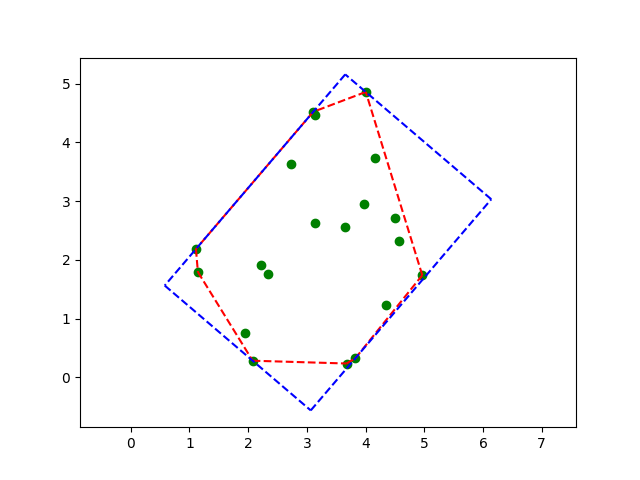
\includegraphics[scale=0.45]{ch1.png}
\caption{Convex hull and bounding rectangle example}
\label{fig:display}
\end{figure}

\item [Testing -- 15 points] \hfil \\
Test your program on a variety of inputs and special cases. Make
sure to test your program on the randomly chosen real-valued
numbers (and not just integers). Can your program fail due to
numerical errors or missed special cases?  Can you predict for
what inputs this may  happen, and what will happen to your
program? (Programs can fail in several ways; some examples: it can
produce a wrong answer, it may produce unpredictable or
contradictory results, or it may simply `die'.) You will also be
provided a standard test set of points that should be handled by
your program.
\end{description}

\subsection*{Submission}
Please use the course website to submit a single  zip  named   FirstName\_LastName\_HW2.zip
The zip archive should contain:  (1) the analysis portion of the assignment,  
(2)  the documented python source file, and 
(3) a PDF readme file  specfying the instructions for running the code.  
It should also include at least 1 sample run with input and output,  and specify any specific dependencies or requirements of your code.  

\end{document}
